\documentclass{school-22.211-notes}
\date{February 29, 2012}

\begin{document}
\maketitle

\topic{Dilution Cross Section/Dilution Factor}
In an infinite homogeneous medium with one resonance absorber and one moderator,  we write removal rates equals scattering rates, 
\begin{align}
\left[ N_r \sigma_r (u) + N_m \sigma_m (u) \right] \phi (u) &= \int_{-\infty}^u N_m \sigma_m (u') \phi(u') P(u' \to u) \du' \\ 
&= N_m \sigma_m \int_{-\infty}^u \phi(u') P(u' \to u) \du' \\
&= N_m \sigma_m C \\
\phi(u) &\propto \frac{N_m \sigma_m}{N_r \sigma_r(u) + N_m \sigma_m} \\
\phi(u) &\propto \frac{ \frac{N_m}{N_r} \sigma_m}{\sigma_r(u) + \frac{N_m}{N_r} \sigma_m}  \label{flux-shape}
\end{align}
In the above derivation we made two assumptions:
\begin{itemize}
\item The moderator's xs is independent of energy near resonances. For almost any moderators we can pick, the assumption that the elastic scattering xs is constant is valid in the thermal range as in Figure~\ref{moderator-sigma-s}. 
\item $\int \phi(u') P(u' \to u) \du'$ is constant. We know that the flux above the resonance is 1/E and hence constant in lethargy. If we assume scattering into the resonance comes from this constant lethargy region, then the resonance lethargy is constant as well. 
\end{itemize}
\begin{figure}
  \centering
  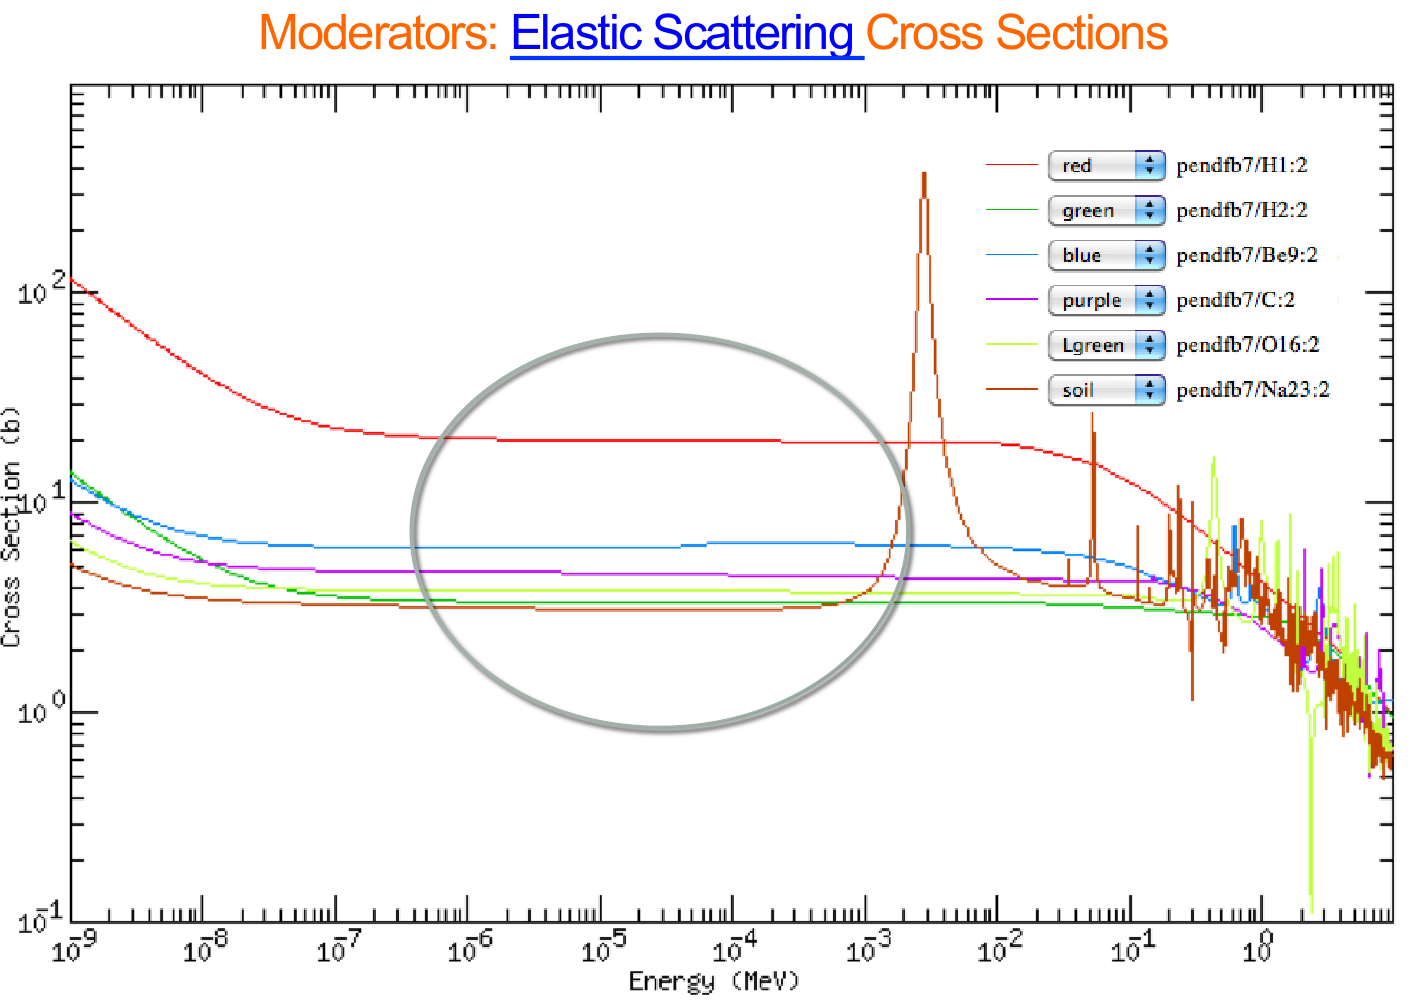
\includegraphics[width=3in]{images/moderator-sigma-s.png}
  \caption{Moderator Elastic Scattering Cross Sections} \label{moderator-sigma-s}
\end{figure}
Eq.~\ref{flux-shape} suggests that \textit{in infinite medium the flux shape near resonance depends only on the ratio of the number density of the moderator to the resonance absorber and the moderator cross section.} But once we move into a finite medium or we take into account leakage, then the absolute number densities are needed.
 
To capture the ratio of number densities and the moderator cross section, we define \hi{dilution cross section} as,
\eqn{ \boxed{ \sigma_d = \frac{N_m \sigma_m}{N_r} } }
Then the flux shape near resonance is,
\eqn{ \boxed{ \phi(u) \propto \frac{\sigma_d}{\sigma_r + \sigma_d} } }
This flux shapes let us to compute approximated effective RI. Recall RI is defined as, $\RI = \int \sigma_r (u) \du$. Then the approximated effective RI is,
\eqn{ \boxed{ \RI_{\eff} = \int \sigma_r(u) \frac{\sigma_d}{\sigma_r + \sigma_d} \du }  }
Two extremes of $\RI_{\eff}$ and $\sigma_d$:
\begin{itemize}
\item As $\sigma_d \to \infty$, the entire media is moderator, we reach the limit of infinite dilute resonance absorption appears, and $\RI_{\eff} \to \RI$; at infinite dilute, we should get within 1\% of the ENDFVII xs data;
\item As $\sigma_d \to 0$, analytically our assumptions do not hold true any more, but the MC is true that as $\RI_{\eff} \to 0, \phi \to 0$ as seen in Figure~\ref{dilution-factor-increase}. Interpretation: as we have no moderator, every atom is self-shield [FIXME]
\end{itemize}
Figure~\ref{dilution-factor-increase} is generated from effective RI of MC calculations at 300K with half a million neutrons, 2 barns hydrogen 1/v absorber. It illustrates that, a) the dilution ratio U/H is related with dilution xs $\sigma_d$ such that they are inversely proportional; b) as the fraction of \ce{^{238} U} increases, U/H increases, $\sigma_d$ decreases, more absorption happens during resonance, hence more flux dips on the spectrum plot and smaller effective RI values in the resonance range. That is, \textit{RI are very dependent on the density of resonant materials.}
\begin{figure}
  \centering
  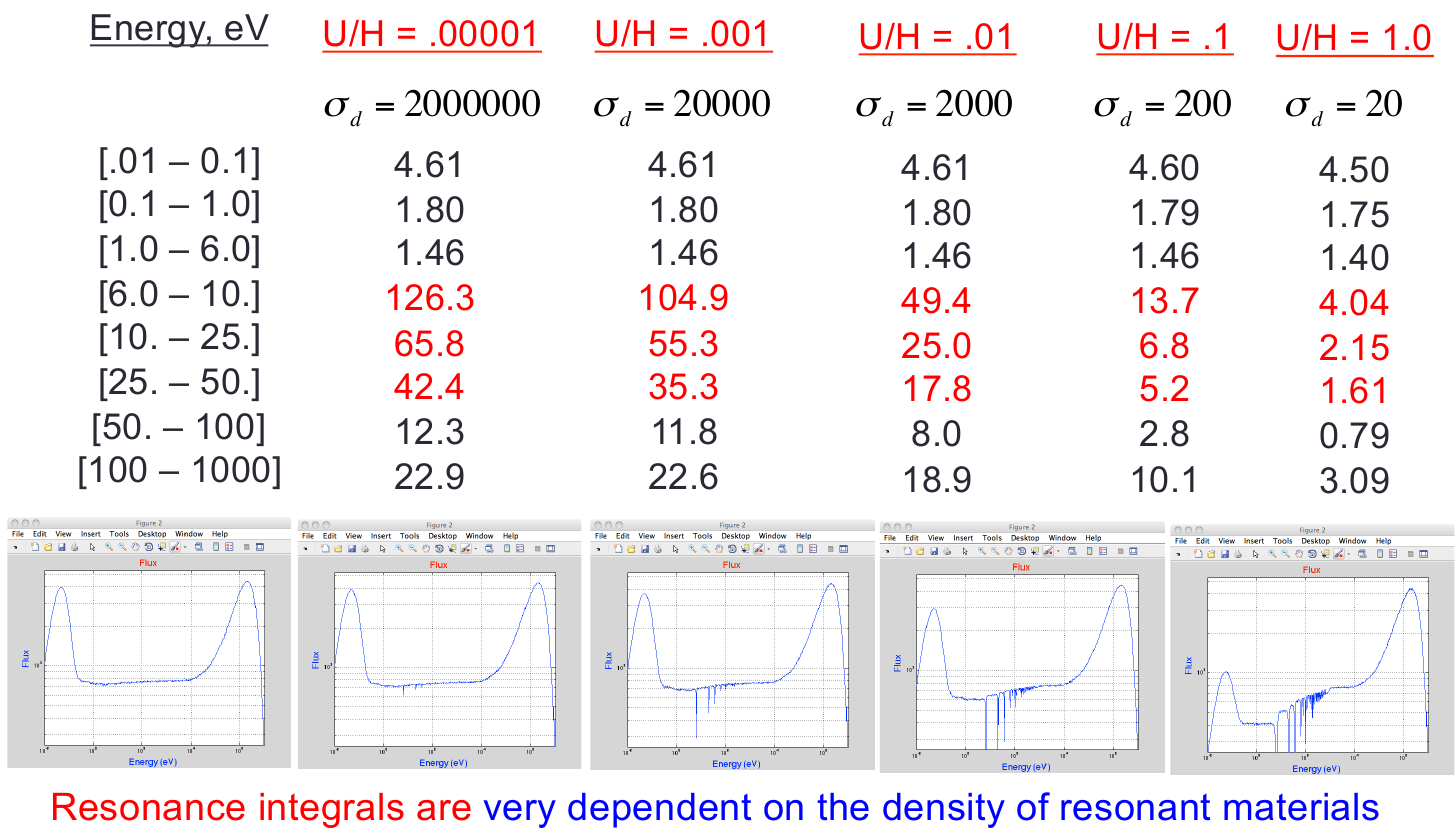
\includegraphics[width=4in]{images/dilution-factor-increase.png}
  \caption{Spectrum Resonance Dips More As U/H Increases and Dilution Cross Section Decreases} \label{dilution-factor-increase}
\end{figure}

The scattering down to resonance is independent of the resonance. In another word, if the spectrum above a resonance returns to 1/E as in Figure~\ref{1overE}, the group cross sections will be independent of higher energy absorptions. 
\begin{figure}
  \centering
  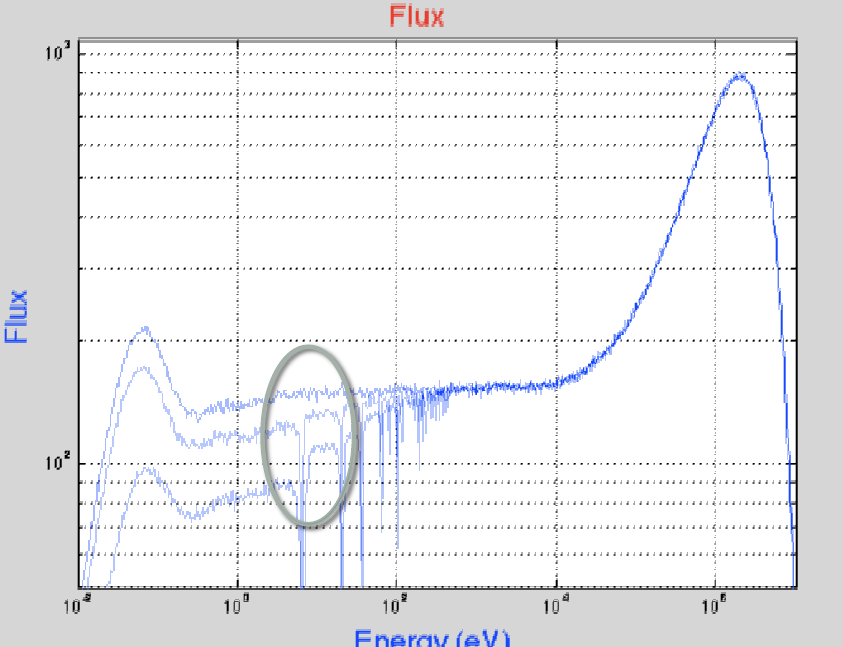
\includegraphics[width=3in]{images/resonance-1-over-E.png}
  \caption{The 1/E Spectrum Above A Resonance Suggests Group XS Independent Of Higher Energy Absorption} \label{1overE}
\end{figure}

\topic{Resonance Escape Probability}
\begin{align}
p &= \exp \left( - \frac{N_R \RI_{\eff}}{\xi \Sigma_m} \right)  = \exp \left( - \frac{\RI_{\eff}}{\xi \sigma_d} \right)
\end{align}
The equation here is an approximation. And for hydrogen systems, we know $\xi \to 1$, hence the resonance escape probability becomes:
\eqn{ p = \exp \left( - \frac{\RI_{\eff}}{\sigma_d} \right) }
That is, \textit{p only depends on effective RI and dilution cross section.} For instance, in a hydrogen system with $\sigma_d = 200$, we can tabulate the p values as in Table~\ref{p-values}. The last entry tells us that \textit{about 20\% of neutrons are absorbed in U238 resonances.}
\begin{table}
  \centering
  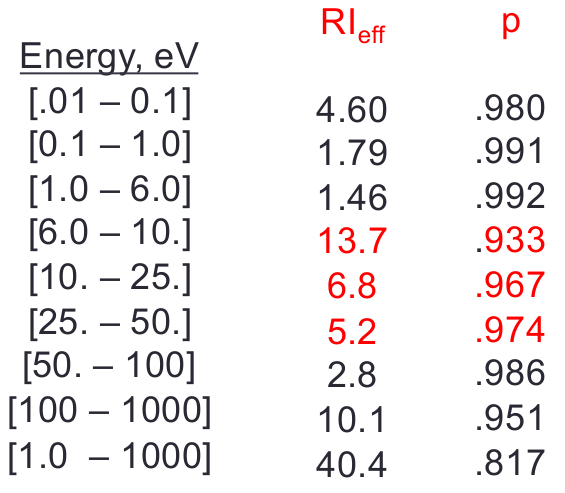
\includegraphics[width=1.5in]{images/resonance-escape-probability.png}
  \caption{Resonance Escape Probability For A Hydrogen System} \label{p-values}
\end{table}
T
The full derivation of resonance escape probability is the following. Assumptions: only elastic down scatter above the resonance, $\sigma_{a,m} = 0, \sigma_{s} = $const, and only a single resonance absorber. 

Start from our balance equation (scattering in = resonance absorption),
\begin{align}
\frac{S}{\zeta(u)} \du &= \left[ N_r \sigma_{a,r} (u) + \Sigma_m \right] \phi(u) \du = N_r \left[ \sigma_{a,r} (u) + \sigma_d \right] \phi(u) \du \\
\Rightarrow \phi(u) &= \frac{S}{\zeta(u) N_r \left[ \sigma_{a,r} (u) + \sigma_d \right] } 
\end{align}
Define resonance escape probability as:
\begin{align}
p &= \frac{S - \int N_r \sigma_a(u) \phi(u) \du}{S} \\
&= 1 - \frac{\int N_r \sigma_a(u) \frac{S}{\zeta(u) N_r \left[ \sigma_{a,r} (u) + \sigma_d \right] } \du }{S} \\
&= 1 - \int \frac{\sigma_{a,r} (u) }{\zeta(u) \left[ \sigma_{a,r} (u) + \sigma_d \right] } \du
\end{align}
If the mean logarithmic energy decrement is independent of lethargy, 
\eqn{ p = 1 - \frac{1}{\zeta} \int \frac{\sigma_{a,r} (u)}{\sigma_{a,r} (u) + \sigma_d} \du }
But using our definition of effective RI,
\eqn{ \RI_{\eff}^{u1 \to u2} = \int_{u1}^{u2} \frac{\sigma_{a,r} (u) \sigma_d}{\sigma_{a,r} (u) + \sigma_d} \du }
We can write $p$ in terms of $\RI$:
\eqn{ \boxed{p^{1\to 2} = 1 - \frac{\RI_{\eff}^{u1 \to u2}}{\zeta \sigma_d} } }
Since the source is incrementally reduce with each successive resonance,
\eqn{ p^{u1 \to uN} = \left( 1 - \frac{\RI_{\eff}^{u1 \to u2}}{\zeta \sigma_d} \right) \left( 1 - \frac{\RI_{\eff}^{u2 \to u3}}{\zeta \sigma_d} \right)
  \cdots \left( 1 - \frac{\RI_{\eff}^{uN-1 \to uN}}{\zeta \sigma_d} \right) }
We approximate the sequence as,
\eqn{ p^{u1 \to uN} = \exp \left( - \frac{\Sum_{u1}^{uN-1} \RI_{\eff}^u}{\zeta \sigma_d} \right) }
or
\eqn{ \boxed{ p \approx \exp \left( - \frac{\RI_{\eff}}{\zeta \sigma_d} \right) = \exp \left( - \frac{N_r \RI_{\eff}}{\zeta \Sigma_m} \right)  } }
which for hydrogen system becomes, 
\eqn{ p \approx \exp \left( - \frac{\RI_{\eff}}{\sigma_d} \right) }


\end{document}
